\section{Introduction}

System identification is the field dedicated to methodologies for deriving models from data.
\begin{figure}[H]
    \centering
    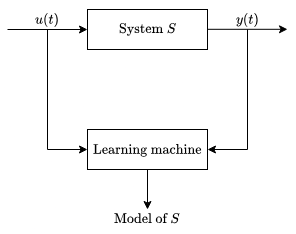
\includegraphics[width=0.5\linewidth]{images/identification.png}
    \caption{Identification process}
\end{figure}
Key characteristics of derived models include:
\begin{itemize}
    \item \textit{Limited validity}: the model can't reveal more about the system than what's inherently present in the data used for its derivation.
    \item \textit{Difficult physical interpretation}: model parameters lack direct physical interpretation; they are conceived to explain data and aren't derived from physical laws.
    \item \textit{Simple derivation and usage}. 
\end{itemize}
The identification process starts with selecting the model class (linear, nonlinear, AR, MA, ARMA). 
However, data provided to the system are imperfect (affected by noise and only partially representative of the phenomena involved) and may have other issues like quantization, missing data, outliers and more.

Additionally, the process may vary over time, rendering an approach solely based on time-invariant models insufficient. 
Furthermore, not all signals and variables relevant to the system are always measurable.

In summary, the fundamental elements of the identification problem are:
\begin{enumerate}
    \item The system $\mathcal{S}$. 
    \item The model family $\mathcal{M}$. 
    \item The identification method $\mathcal{I}$. 
    \item The identification experiment $\mathcal{E}$. 
\end{enumerate}

\subsection{Parametric system identification}
The steps involved in parametric system identification are as follows:
\begin{itemize}
    \item \textit{Experiment design and data collection}: the first phase involves designing and conducting an identification experiment ($\mathcal{E}$) to gather the necessary data. 
        For input-output systems, the system ($\mathcal{S}$) is subjected to an appropriate input signal, and the inputs and outputs are observed and recorded over a period of time. 
        Factors such as the choice of input signal and the length of the data ($N$) impact the informativeness and confidence of the resulting dataset. 
        Data preprocessing is typically performed to address outliers, missing data, trends, periodicity, etc. 
        The experiment design ($\mathcal{E}$) depends on factors such as the input signal selection, the presence of feedback loops, sampling time, and data pre-filtering. 
        Constraints on the experiment may exist due to security reasons or operational limitations under specific conditions.
    \item \textit{Choice of model class}: a parametric model family $M(\vartheta) = \{M(\vartheta), \vartheta \in \Theta\}$ is selected, believed to be flexible enough to explain the data. 
        The set $\Theta$ defines the admissible parameterization. 
        The choice of model class may be guided by data analysis, prior knowledge of the system, or intended use of the model. 
        The identification problem involves determining the appropriate parameters $\vartheta$. 
        Model types include static/dynamic, discrete/continuous-time, linear/nonlinear, time-invariant/time-varying, and internal/external representation. 
        Non-parametric models are also viable options.
    \item \textit{Choice of identification criterion and parameter estimation}: a suitable method (identification algorithm, $\mathcal{I}$) is employed to estimate the unknown model parameters. 
        This typically involves selecting an identification criterion \(J_N(\theta) \geq 0\) and minimizing it with respect to \(\theta\). 
        The choice of identification method ($\mathcal{I}$) depends on the model class. 
        Minimizing $J_N(\vartheta)$ is straightforward for certain classes where it becomes a quadratic function of $\vartheta$, but more challenging for other classes.
    \item \textit{Model validation}: throughout the identification process, crucial assumptions are made, such as the system ($\mathcal{S}$) belonging to the selected model family $M(\vartheta)$ and fixing model orders. 
        Validation involves conducting a quality check on the obtained model. 
        If the model is deemed unsuccessful, assumptions are reevaluated, and the identification process may need to be revisited from steps one, two, or three.
\end{itemize}